Es gibt einige verschiedene Arbeiten die sich um das Thema Cross-Plattform bzw. Multi-Plattform Entwicklung drehen. Die vorgestellten Arbeiten sind oft Veröffenltichungen im Rahmen von Konferenzen oder andere Wissenschaftliche Arbeiten. Im folgenden sollen einige vorgestellt werden und darauf eingegangen werden, was die Arbeiten von dieser unterscheidet und weshalb diese Arbeit wichtig ist.

\subsubsection{A study on approaches to build cross-platform mobile applications and criteria to select appropriate approach - C.P Rahul Raj \& Seshu Babu Tolety}
In ihrer Arbeit stellen Raj und Tolety zunächst die verschiedenen Arten von Cross-Plattform Entwicklungsansätzen vor. Nachdem sie hier einige vor und Nachteile erläutern gehen sie danach über, zu erläutern wie man eine passende Methode auswählt. Dafür unterscheiden sie zunächst nach der Art der Applikation und unterteilen sie in vier Klassen. Serverdaten-, Sensor bzw. Ein-und Ausgabe gestützte, alleinstehende und Client-Server-Applikationen. Im folgenden erklären sie die verschiedenen Klassen und erläutern jeweils, welchen Ansatz sie am ehesten wählen würden und geben hierfür einige Empfehlungen. So empfehlen sie etwa, dass bei Server gestützten Applikationen grundsätzlich einen Web-gestützten Ansatz empfehlen, da dadurch sowohl das User Interface als auch die Geschäfftslogik komplett genutzt werden kann, ohne sie auf den einzelenen Plattformen neu zu schreiben. Sie schränken dabei jedoch ein, dass sobald die Anwendung selber einen Teil an Funktionalität anbieten soll, ein Hybrider Ansatz der best gewählte wäre. Aus diesen Erklärungen und anderen bildeten sie daraufhin die Entscheidungstabelle, die in Abbildung \ref{fig:decision_table_IEEE_related_work} zu sehen ist. Dabei steht der Wert 1 für nicht empfohlen, 2 empfohlen, aber nicht optimale Methode und 3 perfekte Methode.\cite{IEEE_Rahul_Seshu}

Als Fazit erklären sie dann, dass Cross-Plattform Lösungen die bevorzugte Methodik sind, wenn mehrere Plattformen genutzt werden sollen, wenn Entwicklungszeit und Kosten ein kritischer Faktor sind. Sie sagen asußerdem, dass jeder Ansatz seine eigenen Vor und Nachteile hat und somit eine Entscheidung je nach Applikationsart zu treffen ist. \cite{IEEE_Rahul_Seshu}
\begin{figure}[ht]
  \centering
  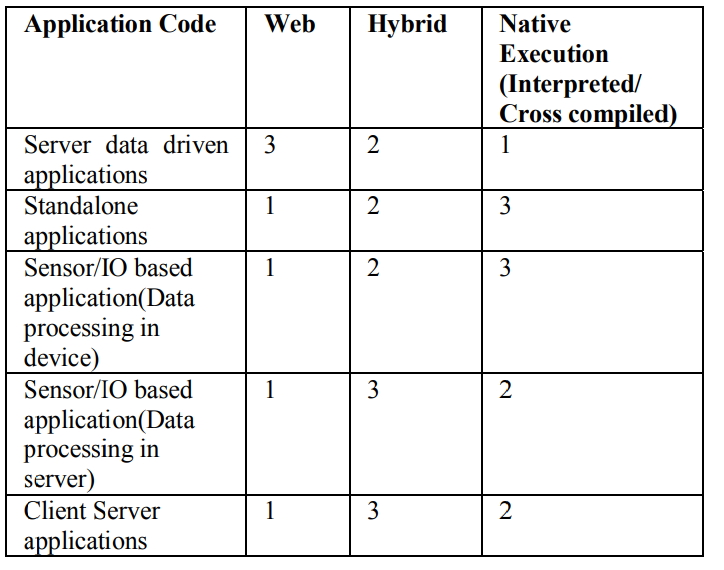
\includegraphics[height=7cm,keepaspectratio]{images/IEEE_related_chapter.jpg} 
  \caption{Entscheidungstabelle für Applikationstyp und bevorzugter Ansatz \cite{IEEE_Rahul_Seshu}}
  \label{fig:decision_table_IEEE_related_work}
\end{figure}

Diese Arbeit stellt einen guten Überblick über einen möglichen Entscheidungsweg dar und erklärt einige wichtige Grundlagen, die zur Unterscheidung bei der Entwicklung von Multi-Plattform-Anwendungen wichtig sind. Jedoch wird einerseits in dieser Arbeit der Aspekt der rein nativen Entwicklung mit den Plattform spezifischen Entwicklungsmethodiken komplett vernachlässigt und die Arbeit stützt sich lediglich auf Recherchen, es wurden jedoch keinerlei Versuche oder messabaren Werte genutzt. Anders ist hier die nächste Arbeit.


\subsubsection{Approaches to mobile application development: Comparative performance analysis - Delia et Al}
Delia et Al vergleichen in ihrer Arbeit die Performance von verschiedenen Ansätzen zur Entwicklung von mobilen Applikationen. Auch sie unterscheiden zunächst, die verschiedenen Klassen der Entwicklungsmethoden. Danach stellen sie ihre Testmethodik vor. Um die Performance der Unterschiedlichen Plattformen zu testen nutzen sie hierfür eine Mathematische Berechnung indem die Summe über 500.000 Schleifendurchläufe einer Berechnung bestehend aus einem Logarithmus, einer Wurzel und Fakultät berechnet wird. Um das ganze etwas differenzierter zu betrachten nutzten sie dafür verschiedene Android und iOS Geräte um die sieben verschiedenen Anwendungen laufen zu lassen. Um die Zeit zu messen, die die Berechnung dauerte, namen sie vor und nach der Ausführung der Berechnung die Zeit und bildeten daraus die Differenz um zu sehen wie lang die jeweiligen Berechnung dauerte. Dies führten sie dann jeweils 30 mal aus und berechneten daraus die Durchschnittliche Laufzeit T und die Standardabweichung S. Das Ergebnis ist in Abbildung \ref{fig:result_table_IEEE_related_work} zu sehen.\cite{IEEE_development_classes}

\begin{figure}[ht]
  \centering
  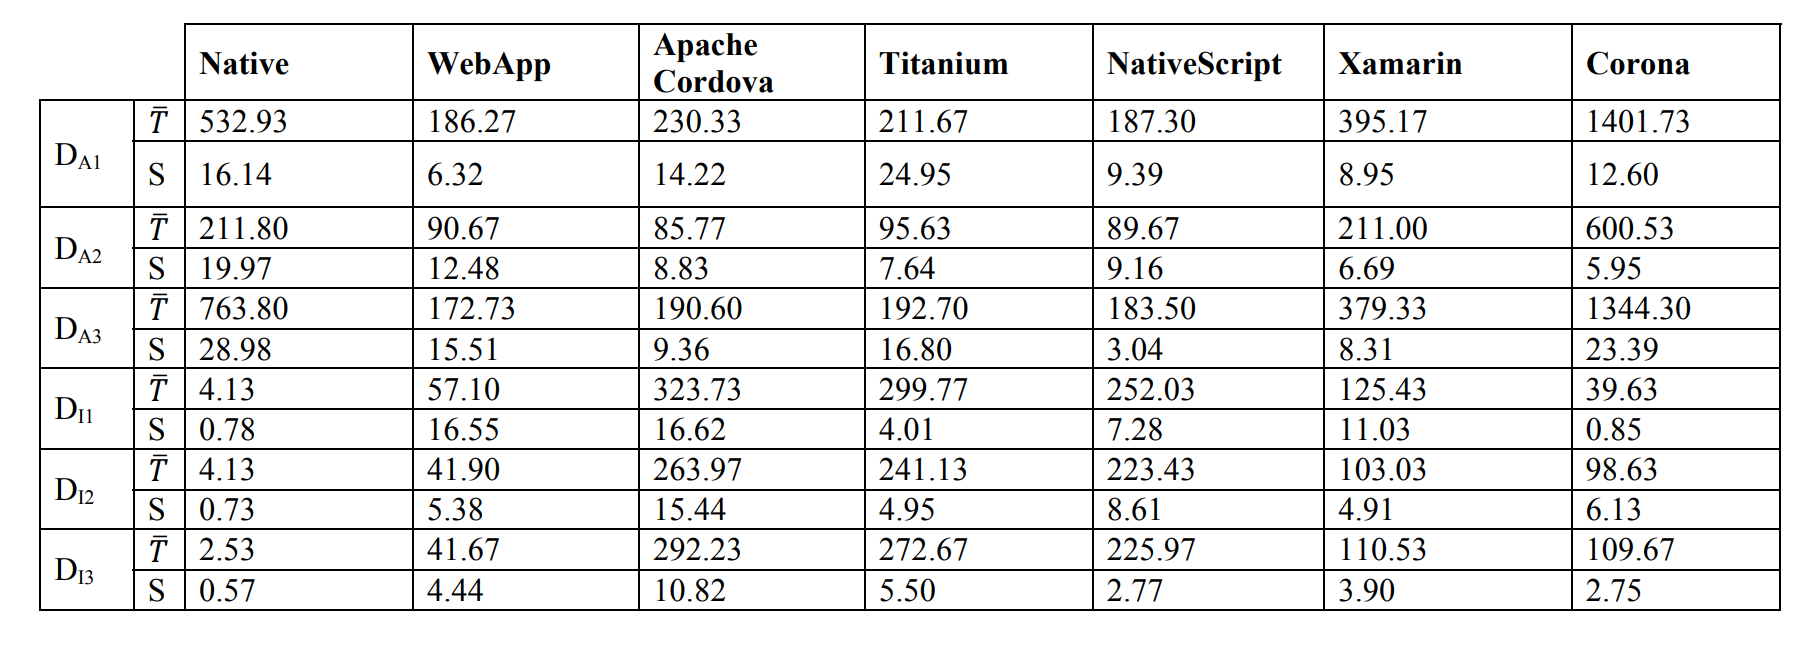
\includegraphics[width=\textwidth,keepaspectratio]{images/IEEE_Delia_Al.png}
  \caption{Ergebnisstabelle der Performancemessungen \cite{IEEE_development_classes}}
  \label{fig:result_table_IEEE_related_work}
\end{figure}

Interessant ist hier vor allem zu sehen, dass es erhebliche Unterschiede zwischen Android und iOS gibt. So ist nicht sichergestellt, dass nur weil ein Ansatz auf Android sehr schnell lief, er auch auf iOS so gut lief. Jedoch erklären sie hierzu selber in der Auswertung ihrer Arbeit, dass ein Vergleich durch die Verwendung verschiedener Hardware schwierig ist.\cite{IEEE_development_classes} Dennoch sagen sie selber, dass die benutzte Implementierung auf iOS effizienter scheint, als die auf Android, was sie auf die Android Runtime zurückführen. Generell stellten sie fest, dass Web-Applikationen in ihren Test die beste Performance über die Geräte hinweg zeigten.\cite{IEEE_development_classes}

In dieser Arbeit wurde lediglich auf die Performance der Applikationen eingegangen. Zu der Webentwicklung gehören jedoch so viel mehr Aspekte, die einen Einfluss auf die Auswahl der Entwicklungsmethode haben. Dazu kommt, dass die Arbeit, da sie 2017 bereits geschrieben wurde, heute komplett anders aussehen könnte/würde. Nicht nur, dass mittlerweile auf beiden Plattformen neue und performantere Programmiersprachen genutzt werden, sondern auch die Geräte von heute haben deutlich schnellere Prozessoren, mehr Arbeitspeicher und vieles mehr. Ein Smartphone von 2017 ist mit einem heutigen nicht mehr vergleichbar. Deswegen rückt der Faktor der Performance immer weiter in den Hintergrun, was auch eine recht neue Untersuchung von 2020 von Bi{\o}rn-Hansen et Al bestätigt. Sie fanden zwar einige Unterschiede zwischen den verschiedenen Frameworks gefunden, kamen aber am Ende zu dem Fazit, dass zwar in der Summe die nativen etwas besser Abschnitten, aber einige hybriden Ansätze in ein paar Aufgaben sogar besser performten als die nativen und kein Ansatz in allen Punkten besser war als die anderen.\cite{BirnHansen.2020}

\subsubsection{Framework Choice Criteria for Mobile Application Development - Khachouch et Al}
Ebenfalls eine neuere Untersuchung ist die folgende von Jhachouch et Al. Ihr Ziel war es dabei einen Entscheidungsgraphen zu erstellen, bei dem man durch Beantwortung einiger Fragen am Ende zu einer Antwort gelangen soll. Sie kritisierten, dass es durchaus einige solcher Graphen gäbe, jedoch dies oft in Richtung eines beworbenen Frameworks manipuliert wären. Deswegen entwickelten sie einen Fragekatalog und Graphen, der keine Aussage zu einem bestimmten Framework oder Technologie einer Firma trifft, sondern dass zu einer Entwicklungsmethodik rät. Das Ergebnis daraus kann man in Abbildung \ref{fig:decision_graph_IEEE_related_work} sehen.\cite{IEEE_Khackouch_Al}

\begin{figure}[ht]
  \centering
  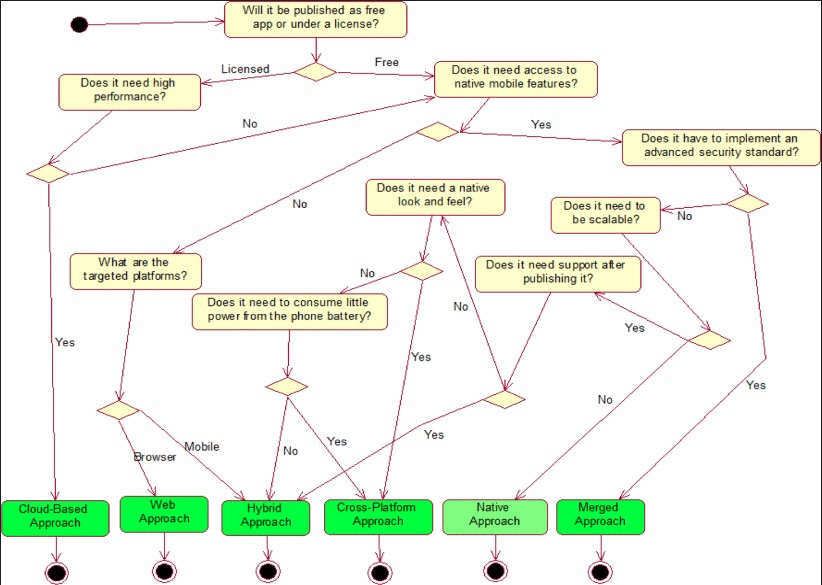
\includegraphics[width=\textwidth,keepaspectratio]{images/IEEE_Khachouch_Decision_Graph.jpg}
  \caption{Entwickelter Entscheidungsgraph von Khachouch et Al \cite{IEEE_Khackouch_Al}}
  \label{fig:decision_graph_IEEE_related_work}
\end{figure}

Sie ziehen am Ende das Fazit, dass wenn "keine Einschränkungen im Bezug auf Kosten oder Personal existieren, der native Ansatz aufgrund seiner Vorteile in Bezug auf Qualität, Leistung und Ergonomie die beste Lösung"\cite{IEEE_Khackouch_Al}{Chapter~4} sei.

\TODO{Nochmal überarbeiten. Noch nicht zufrieden.}
Das Problem an dieser Arbeit ist, dass einerseits es in der Realität es nie den Fall geben wird, dass es keine Einschränkungen bei Kosten oder Personal geben wird. Desweiteren ist es auch dann nicht verständlich, warum etwa ein Cross-Plattform Ansatz nicht auch gut sein könnte. Auch die gestellten Fragen und ihre Anworten sind manchmal etwas irritierend. So ist die Frage ob die Anwendung nach einer Veröffentlichung weiterhin Support benötigt. Bei der Antwort Ja wied der Hybride Ansatz empfohlen bei Nein geht es weiter und nach ein bis zwei Fragen wird dann zwischen Hybriden und Cross-Plattform Ansatz entschieden. Jedoch sollte eine App immer weiter unterstützt beziehungsweise gewartet werden. So sollten etwa Sicherheitsupdates von genutzten Bibliotheken oder sonstiges in Apps eingebaut werden können. Auch die Begründung, warum Cross-Plattform Ansätze ein Support nach der Veröffentlichung hier problematisch ist, erklären sie nicht. Sie sagen sogar in ihrer Erläuterung der Fragen, dass alle von ihnen Untersuchten Ansätze einen guten Support anbieten.\cite{IEEE_Khackouch_Al} Ein Argument der hier angebracht werden könnte, ist, dass Cross-Plattformen stark von ihrer Popularität abhängig sind. So können Frameworks eingestellt werden, wenn sie keine aktive Community mehr haben. Jedoch werden selbst dann oft noch durch Open-Source Unterstützer wichtige Updates veröffentlicht um einen Langzeitsupport zu ermöglichen.